\section{The retarded fast--slow problem and main result}
\label{sec:model-main}

We now fix the model and the local connection whose displacement is studied.
The matrices are chosen so that the critical delay measure is exactly fixed
while one transverse delay channel varies.  Their particular values make the
mechanism transparent and leave all algebraic statements below exact.

\subsection{A two-module FitzHugh--Nagumo equation}

Let \(v=(v_1,v_2)^T\) and \(w=(w_1,w_2)^T\) denote voltage and recovery
variables.  Set
\[
 s_*:=\sqrt{\frac32},\qquad
 r:=\vect{1\\2},\qquad
 \ell:=\vect{1/2\\1/4},\qquad
 P:=r\ell^T,\qquad P_\perp:=\Id-P,
\]
so that \(\ell^Tr=1\).  We study
\begin{equation}
\label{eq:physical-model}
\begin{aligned}
 \dot v(t)={}&F_{\rm FHN}(v(t),w(t))
 +\eps K\bigl[Bv(t)-C_0^\eta v(t-\theta_0/\del)
                    -C_1^\eta v(t-\theta_1/\del)\bigr],\\
 \dot w(t)={}&\eps\vect{v_1(t)-s_*-\mu\\v_2(t)-2\mu}
              -d_wP_\perp\bigl(w(t)-w_*\bigr),
 \qquad \eps=\del^2,
\end{aligned}
\end{equation}
where \(K\in\R\setminus\{0\}\), \(d_w>0\), and
\(0<\theta_0<\theta_1\) are fixed.  The local FitzHugh--Nagumo vector field
and the distinguished equilibrium are
\begin{equation}
\label{eq:FHN-field}
 F_{\rm FHN}(v,w)=\vect{
 v_1-v_1^3/3-w_1+(v_2-v_1)/2\\
 v_2-v_2^3/3-w_2+2(v_1-v_2)},\qquad
 v_*:=\vect{s_*\\0},\quad w_*:=\vect{0\\2s_*}.
\end{equation}
The instantaneous term \(-d_wP_\perp(w-w_*)\) is a fixed transverse
recovery coupling.  It vanishes on the collective recovery line and removes
an additional transverse slow center; it is not a control parameter.

The delayed layers are
\begin{equation}
\label{eq:delay-layers}
 C_0=\mat{1/6&1/12\\1/6&1/4},\qquad
 C_1=\mat{1/3&1/6\\1/2&5/12},\qquad
 T=\mat{1&0\\-2&0},
\end{equation}
The redistributed layers and their total gain are
\nopagebreak[4]
\begin{equation}
\label{eq:eta-layers}
 C_0^\eta=C_0+\eta T,\qquad
 C_1^\eta=C_1-\eta T,\qquad
 B=C_0+C_1.
\end{equation}
Although \(T\) is signed, the two physical layers remain entrywise positive
for
\begin{equation}
\label{eq:eta-positive}
 -\frac16<\eta<\frac1{12}.
\end{equation}
Thus \(\eta\) is a tangent direction through a positive layer family rather
than a signed coupling layer by itself.

The feedback gain in \cref{eq:physical-model} is weak, of order \(\eps\),
whereas the physical delays are long, of order \(\eps^{-1/2}\).  Passing to
the fold time \(s=\del t\) makes the delay translations fixed:
\[
 \del(t-\theta_k/\del)=s-\theta_k.
\]
Consequently all local history maps below act on the fixed Banach space
\begin{equation}
\label{eq:history-space}
 \cC:=C([ -\theta_1,0],\R^4),\qquad
 \norm{\phi}_{\cC}=\max_{-\theta_1\le\vartheta\le0}\abs{\phi(\vartheta)}.
\end{equation}
Here \(\cC\) is written in the scaled chart variables
\((X,Y,Z,W)\).  For every fixed \(\del>0\), the affine blow-up
\cref{eq:blowup-scaling} and the time change \(s=\del t\) give a
bijective identification with physical histories on
\([ -\theta_1/\del,0]\).  Equality in \(\cC\) is therefore equality of
the corresponding complete histories of the original RFDE, not merely
equality of their current states.
The obstacle is therefore not a growing rescaled history interval.  It is
the singular transverse rate generated by the fixed coupling together with
the need to compare complete histories through a nonhyperbolic fold.

\subsection{What the critical projection does not see}

The next proposition collects the exact algebra that motivates the theorem.
Put
\[
 q:=\vect{1\\-2},\qquad m:=\vect{1/2\\-1/4}.
\]
Then \((r,q)\) and \((\ell,m)\) are biorthogonal bases.

\begin{proposition}[Fixed critical delay measure]
\label{prop:fixed-measure}
For every \(\eta\) satisfying \cref{eq:eta-positive}, the following hold.
\begin{enumerate}[label=\textup{(\roman*)}]
\item The constant history \((v_*,w_*)\) is an equilibrium of
      \cref{eq:physical-model} at \(\mu=0\).
\item The fast voltage Jacobian is
\[
 A_0=D_vF_{\rm FHN}(v_*,w_*)=-2P_\perp,\qquad
 A_0r=0,\quad A_0q=-2q,\quad \ell^TA_0=0.
\]
Moreover
\[
 \ell^TD_v^2F_{\rm FHN}(v_*,w_*)[r,r]=-s_*\ne0,\qquad
 \vect{v_1-s_*-\mu\\v_2-2\mu}=r(X-\mu)
\]
on the line \(v=v_*+rX\).  Hence this line contains a nondegenerate fold
with scalar unfolding parameter \(\mu\).
\item The total delayed gain and the complete delay measure seen by the
critical projection are independent of \(\eta\):
\begin{align}
 C_0^\eta+C_1^\eta&=B, & Br&=r,
 \label{eq:total-gain}\\
 \ell^T\mathbb B_\eta(\dd\theta)r
 &=\frac13\delta_{\theta_0}(\dd\theta)
   +\frac23\delta_{\theta_1}(\dd\theta),
 &
 \mathbb B_\eta&:=C_0^\eta\delta_{\theta_0}
                  +C_1^\eta\delta_{\theta_1}.
 \label{eq:projected-measure}
\end{align}
\item The transverse delay measure is not fixed:
\begin{equation}
\label{eq:transverse-measure}
 P_\perp\mathbb B_\eta(\dd\theta)r
 =\eta q\bigl[\delta_{\theta_0}(\dd\theta)
               -\delta_{\theta_1}(\dd\theta)\bigr].
\end{equation}
Equivalently, for a scalar critical history \(x\),
\begin{equation}
\label{eq:history-projections}
\begin{aligned}
 \ell^T\cH_\eta[rx]
 &=x(0)-\frac13x(-\theta_0)-\frac23x(-\theta_1),\\
 P_\perp\cH_\eta[rx]
 &=\eta q\,[x(-\theta_1)-x(-\theta_0)],
\end{aligned}
\end{equation}
where
\(
 \cH_\eta[rx]=Brx(0)-C_0^\eta r x(-\theta_0)
                         -C_1^\eta r x(-\theta_1).
\)
\end{enumerate}
\end{proposition}

\begin{proof}
The identity \(B-C_0^\eta-C_1^\eta=0\) makes the feedback vanish on
constant histories.  Direct differentiation of \cref{eq:FHN-field} gives
\[
 A_0=\mat{-1&1/2\\2&-1}=-2P_\perp,
\]
and the stated fold curvature follows from the two cubic voltage terms.
The four \(\eta\)-dependent entries are
\(
1/6+\eta,1/6-2\eta,1/3-\eta,1/2+2\eta
\), whose positivity is equivalent to \cref{eq:eta-positive}.
Finally, \(Tr=q\), \(\ell^Tq=0\), and direct multiplication gives
\(
 \ell^TC_0^\eta r=1/3
\) and
\(
 \ell^TC_1^\eta r=2/3
\).
These identities yield \cref{eq:projected-measure}--\cref{eq:history-projections}.
\end{proof}

The proposition exhibits the mechanism in its sharpest form.  Any scalar
model retaining only the critical projection sees exactly the same delayed
operator for all \(\eta\).  The full system does not: the delay redistribution
first excites \(q\), and the nonlinearity later returns that response to the
critical direction.

\begin{figure}[t]
\centering
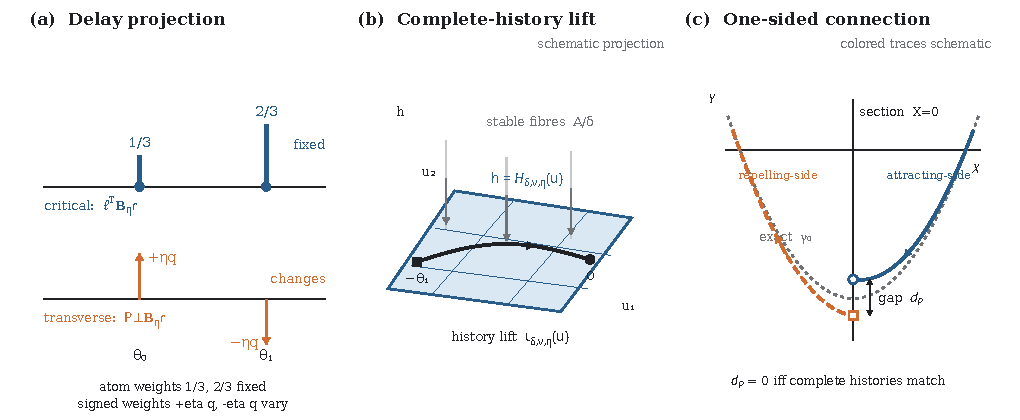
\includegraphics[width=.98\textwidth]{figures/figure1_mechanism.pdf}
\caption{Mechanism behind the threshold displacement.  Redistributing the
two positive delay layers leaves both their total gain and the complete
critical projected delay measure unchanged.  The same redistribution creates
a transverse history forcing, whose stable response is returned by the cubic
nonlinearity to the critical direction and shifts the complete-history
connection.}
\label{fig:mechanism}
\end{figure}

\subsection{Fold coordinates and the singular canard}

Let \(\alpha=s_*/2=\sqrt6/4\).  In modal coordinates we use the anisotropic
scaling
\begin{equation}
\label{eq:blowup-scaling}
\begin{aligned}
 v(t)&=v_*+\del rX(s)+\del^2qZ(s),\\
 w(t)&=w_*-\del^2rY(s)+\del^4qW(s),\\
 \mu&=\del^2\nu,\qquad s=\del t.
\end{aligned}
\end{equation}
The transverse recovery variable is of order \(\del^4\); this is the scale
on which the fixed recovery coupling and the weak delayed return balance.
The exact transformed RFDE is written in \cref{sec:fold-jet}.  At
\(\del=0\), its stable algebraic variables satisfy
\begin{equation}
\label{eq:singular-stable-graph}
 Z_0=-\frac{\alpha}{2}X^2,\qquad
 W_0=-\frac{\alpha}{2d_w}X^2,
\end{equation}
and the critical variables solve
\begin{equation}
\label{eq:singular-critical-system}
 X'=Y-\alpha X^2,\qquad Y'=-X.
\end{equation}
Its distinguished entire solution is
\begin{equation}
\label{eq:singular-canard}
 \gamma_0(s)=\vect{X_0(s)\\Y_0(s)}
 =\vect{-s/(2\alpha)\\(s^2-2)/(4\alpha)}.
\end{equation}

The local construction uses a logarithmic half-length
\begin{equation}
\label{eq:Sdelta}
 S_\del=\sqrt{2p\log(1/\del)}.
\end{equation}
The estimates below first produce a finite threshold \(p_*>4\), depending
only on the fixed derivative orders and tame exponents.  We then fix
\(p>p_*\) once and for all, before choosing \(\del_0\).  This order of
quantifiers prevents the endpoint suppression from being circular.  We also
fix an additional amount of flow and delay buffer.  A
\emph{preparation datum} \(\cP\) consists of this fixed \(p\), the buffer,
parameter-independent smooth cutoff profiles for the history graph and the
prepared planar field, a fixed degree-three extension in the normal
coordinate, and the two tail conditions used in the one-sided problem.  We
call \(\cP\) admissible if the cutoffs agree with the uncut RFDE on the full
continuous flow hull of the shrinking tube around
\(\gamma_0([-S_\del,S_\del])\), agree with \cref{eq:singular-critical-system}
near the prepared endpoints, and have the common finite derivative bounds
specified in \cref{def:admissible-preparation}.  The preparation selects a local
connection; it does not modify the retained histories on the uncut tube.

For each fixed admissible \(\cP\), \cref{sec:history-graph,sec:connection}
constructs two one-sided histories, denoted \(z^a_\cP\) and \(z^r_\cP\),
which meet the common section \(X=0\).  Their scalar normal gap is denoted
\(\mathfrak d_\cP(\del,\nu,\eta)\).  The normalization is chosen so that
\begin{equation}
\label{eq:gap-equivalence-preview}
 \mathfrak d_\cP=0
 \quad\Longleftrightarrow\quad
 z^a_\cP(0)=z^r_\cP(0)
 \quad\Longleftrightarrow\quad
 \iota_{\del,\nu,\eta}(z^a_\cP(0))
 =\iota_{\del,\nu,\eta}(z^r_\cP(0))\ \hbox{in }\cC,
\end{equation}
where \(\iota_{\del,\nu,\eta}\) is the injective complete-history embedding.
Thus the
root is a history connection rather than a zero of a chosen experimental
observable.

\subsection{Main theorem}

We can now state the result.  Fixing a preparation always means first
fixing its profiles, buffers, and extension operator, then choosing the
logarithmic exponent above the finite threshold produced by their tame
bounds.  The exact finite-\(\del\) root is not claimed to be
preparation-independent.

\begin{theorem}[Transverse-delay displacement of the canonical connection]
\label{thm:main}
Fix \(K\ne0\), \(d_w>0\), \(0<\theta_0<\theta_1\), and
\(0<\bar\eta<1/12\).  Set
\[
 \nu_0=-\frac{11}{24\alpha}.
\]
For every fixed admissible preparation skeleton in the sense of
\cref{def:admissible-preparation}, there is \(p_*>4\).
Fix \(p>p_*\) and write \(\cP\) for the resulting preparation.  Then there
are \(\del_0,\eta_0,c_0,C>0\), with \(\eta_0\le\bar\eta\), such that,
whenever
\[
 0<\del\le\del_0,\qquad \abs{\eta}\le\eta_0,
\]
the gap \(\mathfrak d_\cP\) has all rectangular derivatives
\(\partial_\nu^i\partial_\eta^j\mathfrak d_\cP\) for
\(0\le i\le1\), \(0\le j\le2\), continuously on
\begin{equation}
\label{eq:root-neighborhood}
 \abs{\nu-\nu_0}\le c_0.
\end{equation}
It satisfies \cref{eq:gap-derivative-preview} and
\[
 \frac{\mathfrak d_\cP}{\del}
 =\sqrt{2\pi}(\nu-\nu_0)+O(\del),\qquad
 \partial_\nu\mathfrak d_\cP\ge\frac{\sqrt{2\pi}}2\del.
\]
Consequently it has exactly one root
\(\nu_{c,\cP}(\del,\eta)\) in \cref{eq:root-neighborhood};
for each fixed \(\del\), this root is \(C^1\) in \(\eta\), and
\(\nu_{c,\cP}=\nu_0+O(\del)\).
At this root the two retained complete RFDE histories coincide and form one
local orbit through the fold chart.  With
\(\mu_{c,\cP}=\del^2\nu_{c,\cP}\),
\begin{equation}
\label{eq:main-law}
\boxed{
 \mu_{c,\cP}(\del,\eta)-\mu_{c,\cP}(\del,0)
 =\frac{K(\theta_0-\theta_1)}{4\alpha}\del^3\eta
  +O(\del^4\abs{\eta}+\del^3\eta^2).}
\end{equation}
The \(O\)-constant depends only on the fixed physical data and the finite
bounds of \(\cP\), not on \(\del,\eta,\nu\).  The same constant can be
chosen for a class of preparations with a common fixed \(p\), supports,
buffers, derivative bounds, and extension-operator norms.  Since
\(4\alpha=\sqrt6\), the leading
coefficient equals \(K(\theta_0-\theta_1)/\sqrt6\).
\end{theorem}

The striking point is the combination of
\cref{eq:projected-measure,eq:main-law}.  All delay information visible to
the critical projection is identical along the \(\eta\)-family, yet the
local connection shifts at order \(\del^3\eta\).  The sign is the sign of
\(K(\theta_0-\theta_1)\); for positive gain and
\(\theta_0<\theta_1\), increasing \(\eta\) moves the root toward smaller
\(\mu\).

The proof has four steps.  First, the singular stable variables are removed
by a complete-history graph that remains regular as \(\del\to0\).  Second,
mixed parameter jets of this graph are continued to the logarithmic tube
sampled by the long delays.  Third, explicit one-sided Green operators remove
the tangent phase and the normally growing Gaussian mode.  Finally, the
normalized gap derivatives are
\begin{equation}
\label{eq:gap-derivative-preview}
\begin{aligned}
 \partial_\nu\mathfrak d_\cP
 &=\sqrt{2\pi}\,\del+O(\del^2),\\
 \partial_\eta\mathfrak d_\cP
 &=-\frac{K(\theta_0-\theta_1)}{4\alpha}
   \sqrt{2\pi}\,\del^2
   +O(\del^3+\del^2\abs{\eta}),\\
 \partial_{\eta\eta}\mathfrak d_\cP&=O(\del^2),
\end{aligned}
\end{equation}
so the implicit-function theorem gives \cref{eq:main-law}.

\begin{remark}[Physical outer selections]
\label{rem:physical-outer}
The preparation is a local selection rule.  If a separately constructed
physical attracting/repelling Fenichel history family enters the retained
graph with parameter-coherent boundary jets bounded by
\(C\langle S_\del\rangle^m\e^{cS_\del}\), then Gaussian endpoint
suppression transfers the leading coefficient in \cref{eq:main-law} to that
physical root.  Such a bound is not proved here for an arbitrary outer
selection, so \cref{thm:main} is not stated as a global maximal-canard or
spiking-threshold theorem.
\end{remark}
